%Experimental Results and Analysis – in this section, you should show the quantitative results – charts and tables. Analyze the results by explaining and highlighting what is important on them in terms of your goals and what is bad. You should explain the strange results too.

%V ďalšej časti prezentujte vlastný prínos a vlastné výsledky porovnajte s výsledkami iných. Charakterizujte použité metódy.
%Vyhýbajte sa používaniu žargónu.
%Používajte starú múdrosť: 1 obrázok je viac než 1000 slov.

\subsection{4-2-4 Encoder} 
\label{sec:results-auto4} 

%==================================================================
\label{sec:results-auto4-introduction} 
In this section, we analyse performance of TLR~(\ref{sec:our-tlr}) for a broad range of parameters $\lambda_h$ and $\lambda_v$. The network architecture is only 4-2-4~(\ref{sec:datasets-auto4}) what allows us to run plethora of simulations. There were two kinds of simulations. First are \emph{two dimensional maps (TDM)}, where $\lambda_v$ is plotted on the $x$ axis, $\lambda_h$ on the $y$ axis and color is used for the $z$ axis. Second are \emph{timelines} which plot success rate to epoch for the best configuration found by TDM. To create TDM we ran 500 networks for each pair ($\lambda_v$, $\lambda_h$) and for timelines we ran 10000 networks. After the simulations ended, the average for each configuration was plotted. The networks were trained while $patSucc^F \neq 1$ or $epoch < Epoch_{\rm max}$. The $Epoch_{\rm max}$ was set to 100,000 in TDM and 1,000,000 in timelines. Note that most of the plots are in \emph{logarithmic} scale. 

%============================================================

\subsubsection{Comparison} 
\label{sec:tlr-auto4-cmp} 

In the following table~(\ref{tab:results-cmp-auto4}) we can see the comparison of the most important models which we analysed on the \emph{4-2-4 encoder} task. We achieved an improvement of BAL $patSucc^F$ from $62.7\%$ to $93.1\%$ by using two different learning rates~(\ref{sec:our-tlr}). This result was improved further to $99.86\%$ by preselecting networks based on initial weights~(\ref{sec:sim-exp-candidates}). This proved that hidden distance and representation convexity are important attributes of BAL~(\ref{sec:results-candidates}). 

On the other hand, many of the analysed models achieved poorly. Notably we tried modified GeneRec learning rules~(\ref{sec:models-generec-modifications}) on BAL, calling this model \emph{BAL GeneRec Learning Rules (BAL GLR)}. This led to no good results. Also, \emph{BAL-recirc}~(\ref{sec:our-bal-recirc}) achieved worse than BAL. We experimented with \emph{momentum} in section~(\ref{sec:results-momentum}), symmetric version of BAL in section~(\ref{sec:our-bal-sym}) and other modification but all without significant improvement in success. 

\begin{table}[H] 
  \centering
    \begin{tabular}{|l|l|l|l|l|}
    \hline
    Algorithm (section)&$\lambda_h$&$\lambda_v$&$patSucc^F$ &Epochs\\ %&SEM(success) \\
    \hline
    BP~(\ref{sec:models-bp}) &2.4 &2.4 &100&60\\ %&5.1\\
    \hline
    GR~(\ref{sec:models-generec}) &0.6 &0.6 &90&418\\ %&28\\
    \hline
    GR Sym~(\ref{eq:models-generec-learning-rule-sym}) &1.4 &1.4 &56&88\\ %&2.9\\
    \hline
    GR Mid~(\ref{eq:models-generec-learning-rule-mid}) &2.4 &2.4 &92&60\\ %&3.4\\
    \hline
    CHL~(\ref{sec:models-chl}) &1.2 &1.2 &56&77\\ %&1.8\\
    \hline
    BAL~(\ref{sec:models-bal})&0.9 &0.9 &62.7& 5136.11\\ %&2.0e+08\\
    \hline
    BAL TLR~(\ref{sec:our-tlr})&0.0002  & 500&93.12&5845.01\\ %&1.52e+08\\
    \hline
    BAL TLR Can~(\ref{sec:sim-exp-candidates})&0.0002&500&99.86&150.417\\ %&5,070,000\\
    \hline
    BAL Recirc~(\ref{sec:our-bal-recirc})&0.0001&1.0&36.0&1221.6\\ %&4.31e+07\\
    \hline
    BAL GLR~(\ref{sec:models-generec-modifications})& any & 0 & 0 & N/A \\ 
    \hline 
    %TODO Symmetric BAL 
    \end{tabular}
  \caption{Comparing performance of different models on the \emph{4-2-4 encoder} task. Data for BP, GR, GR Sym, Gr Mid and CHL are taken from~\citet{o1996bio}.} 
  \label{tab:results-cmp-auto4}
\end{table}

Note that when comparing runtime in table~\ref{tab:results-cmp-auto4} based on \emph{epochs} we must be aware of that GeneRec and BAL-recirc epochs take longer than others. That is because the recirculation step~(\ref{sec:models-generec-activation}) where usually about 5--15 iterations are necessary for activation to settle~(\ref{sec:generec-fluctuation}). Thus the 418 epochs of GeneRec are comparable to the 5845 epochs of TLR in terms of compuration time. 
 

%============================================================
\subsubsection{Two learning rates} 
\label{sec:tlr-auto4}

In Figure~\ref{fig:results-tlr-auto4-performance} we compare success rate for range of $\lambda_v$ and $\lambda_h$. It~is interesting that the subspace with best achieving networks is around the half line $[(10, 0.001),\,(10^9, 0.001)]$. That means the performance mainly depends on $\lambda_h$ while a constraint on $\lambda_v$ is added. Also see the plot for epochs, where a \emph{ridge} occurred around line $[(0.01, 0.0002),\,(10^9, 0.0002)]$. Unfortunatelly, we can only guess what is the reason behind this ridge. Maybe it~is related to $Epoch_{\rm max}$ and the fact that we are calculating epochs only from successful networks. Therefore, successful networks having $\lambda_h < 10^{-6}$ need to converge using $\lambda_v$, because otherwise they would fail to converge because of $\lambda_h \cdot Epoch_{\rm max} < 1$. 

Note that the success space is robust and therefore it is possible to find it by stochastic methods such as Monte Carlo as an additional parameters is introduced. This approach is needed as finding the optimal values of $\lambda_v$ and $\lambda_h$ could take long using the trivial exhaustive search. 

%======== (3D) L1 x L2 x epochs =========
%======== (3D) L1 x L2 x patSuccF =========
\begin{figure}[H]
  \centering
  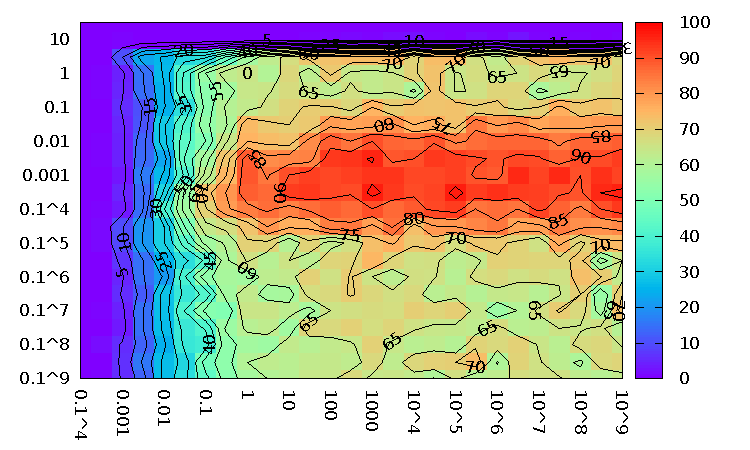
\includegraphics[width=0.49\textwidth]{img/tlr-auto4-success.pdf}   
  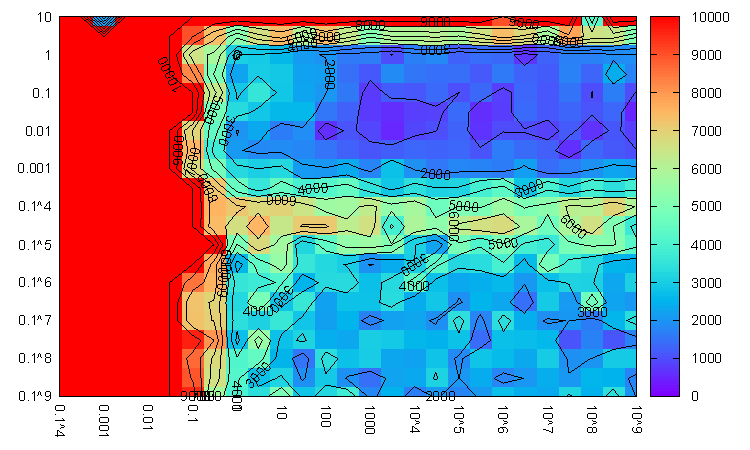
\includegraphics[width=0.49\textwidth]{img/tlr-auto4-epoch.pdf}     
  \caption{TLR success rate and convergence time needed for successful networks on the \emph{4-2-4 encoder} task with $\sigma = 2.3$ and $\mu = 0.0$. Best network achieved $96.5\$$ with $\lambda_h=0.0003$ and $\lambda_v=1000.0$.}
  \label{fig:results-tlr-auto4-performance}
\end{figure}

Note the inconsistency between Table~\ref{tab:results-cmp-auto4}, where 93.12\% success rate was stated for TLR, and in Figure~\ref{fig:results-tlr-auto4-performance} where it was 96.5\%. This is explained by the \emph{law of big numbers}. In the first case the average performance of 10000 networks were used, thus the result is likely to mirror the reality. In the second case only 200 networks were used for a particular $(\lambda_v,\,\lambda_h)$ pair. As there were about 50 candidates for best success rate, it was likely that some of them will achieved better than average. 

\label{sec:our-o-fb-dist-diff}
In Figure~\ref{fig:results-tlr-auto4-epoch} the success timeline for TLR with best $\lambda_h$ and $\lambda_v$ is analysed. We see that the success rate increases even after $10^5$ epochs and our intuition tells us that it will continue even after $10^6$ epochs. Another observation is that $patSucc^B$ first follows $patSucc^F$ for about 100 epochs, but then it stagnates at rate $\approx0.8$. We find this hard to explain as both the architecture and data are symmetric. %OPT

%======== (2D) best TLR on ALL_SUCC x epoch (std-dev) ==========
\begin{figure}[h]
  \centering
  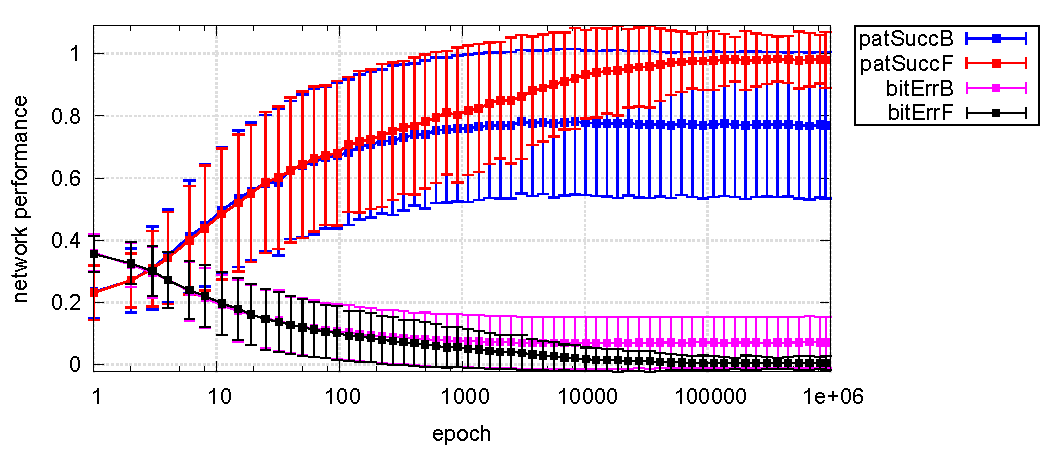
\includegraphics[width=0.8\textwidth]{img/tlr-auto4-best-perf.pdf}\\
  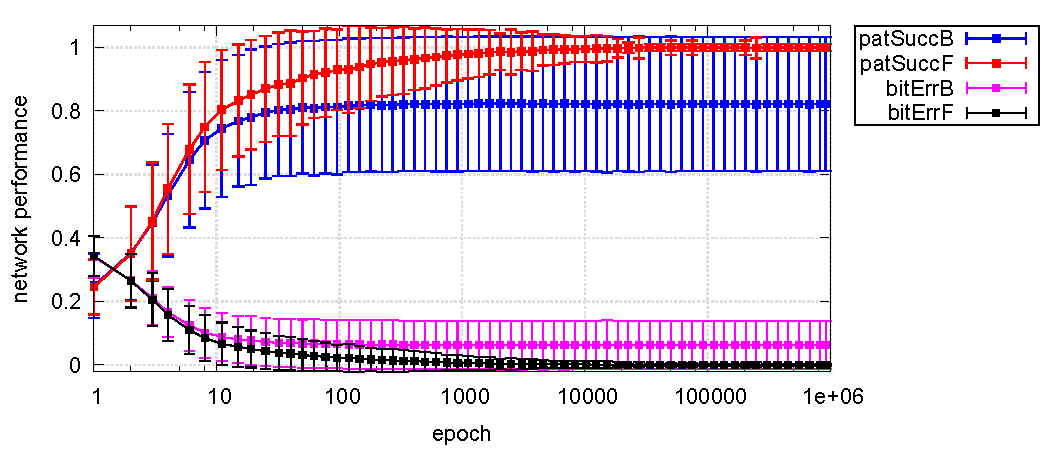
\includegraphics[width=0.8\textwidth]{img/tlr-auto4-best-can.pdf}      
  \caption{TLR success rate timeline for the \emph{4-2-4 encoder} task with $\lambda_h=0.0002$ and $\lambda_v=500$. The top plot without candidate selection and the bottom plot with candidates selection.}
  \label{fig:results-tlr-auto4-epoch} 
\end{figure}

%============================================================
\subsubsection{Hidden activations} 
\label{sec:tlr-auto4-hidden}

In Figure~\ref{fig:results-hidden-activations-bal} and in Figure~\ref{fig:results-hidden-activations-tlr} we show forward hidden activations. Each color represents the forward hidden representation of one of the four inputs in the \emph{4-2-4 encoder} task. As the hidden layer size is 2 then the hidden activation can be mapped to the two dimensional space. The plotted activations start at $epoch=0$ where the starts are depicted with black squares and continue as outlined by the the lines. 

The main difference between TLR and BAL seems to be the speed of activation change. For BAL, as shown in Figure~\ref{fig:results-hidden-activations-bal}, we have a step of size 0.6, which corresponds to four, one for each input, weight updates. Another observation is that after some initial steps BAL tends to stop the activation change. This could be contributed to settling $|H^F-H^B| \approx 0$ as discussed in Section~(\ref{sec:our-hidden-activation}). 

Another source of error could be \emph{non--convex} hidden activation initializations. In the beginning, the weight matrices are initialized by random and that leads to random hidden activations. And if the hidden activations are also non--convex in the end then it~is impossible to perfectly classify on the hidden--to--visible layer due the linear separability theorem discussed in Section~\ref{sec:models-perceptron}. Therefore if the network had non--convex hidden activations in the beginning, then it must \emph{escape} the non--convex state.

%===== hidden activation timelines with commentaries (for TLR, BAL, GeneRec) 
% 2x success, 2x error (wrong settle, divergence) 

\begin{figure}[H]
  \centering
  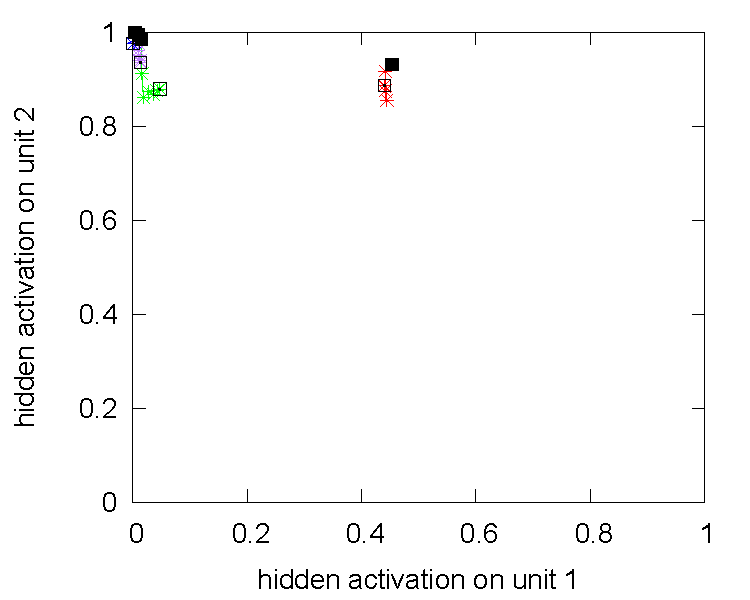
\includegraphics[width=0.45\textwidth]{img/hid-bal-bad-init.pdf}  
  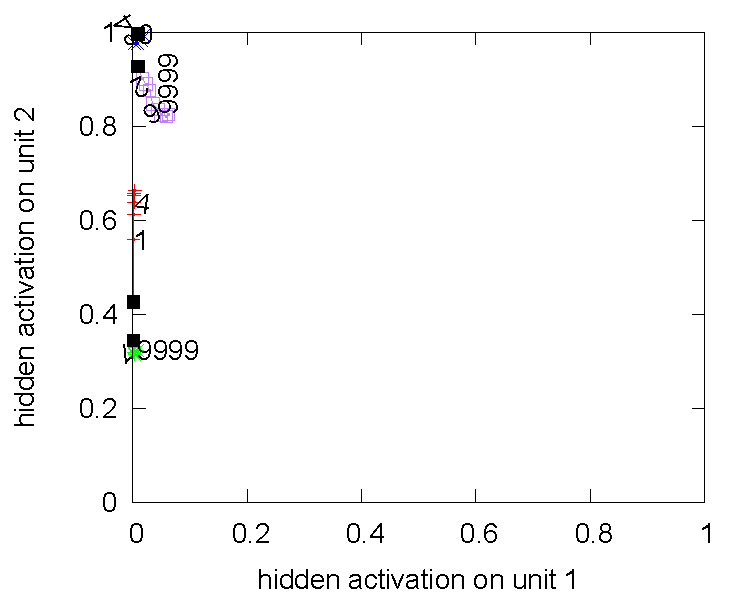
\includegraphics[width=0.45\textwidth]{img/hid-bal-bad-convex.pdf}  \\
  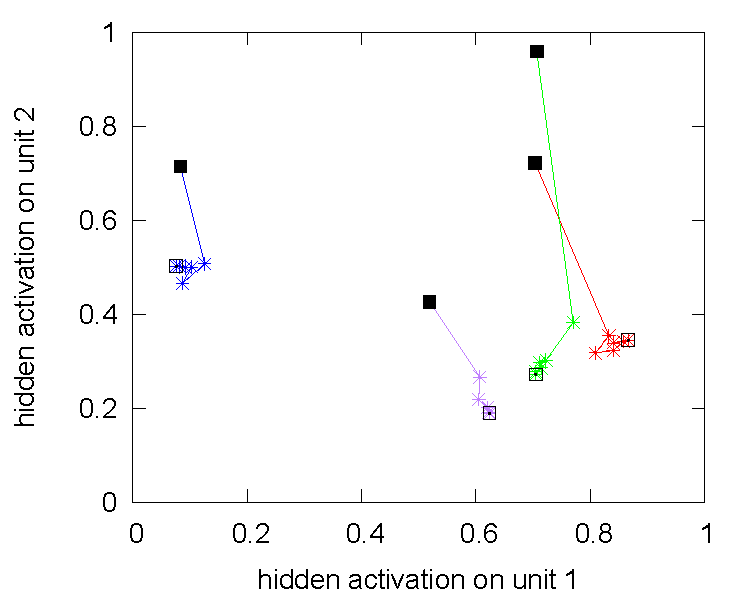
\includegraphics[width=0.45\textwidth]{img/hid-bal-bad-step.pdf}  
  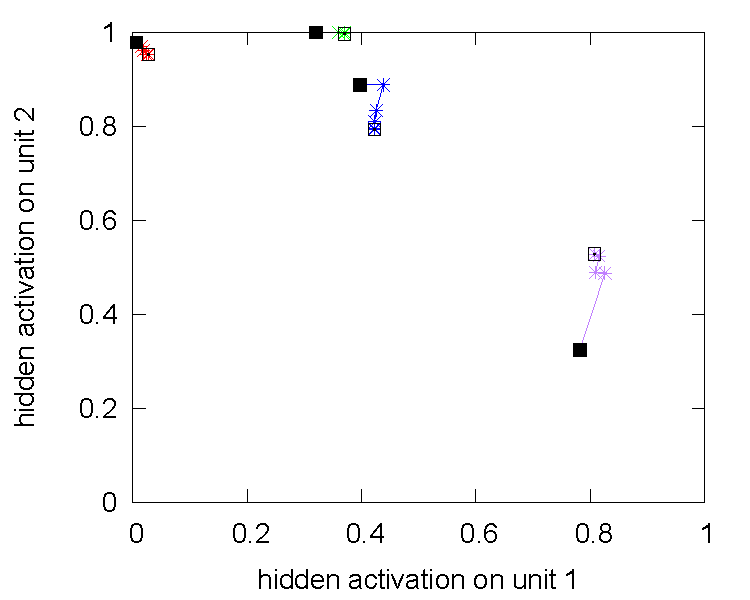
\includegraphics[width=0.45\textwidth]{img/hid-bal-bad-stagnation.pdf}  \\
  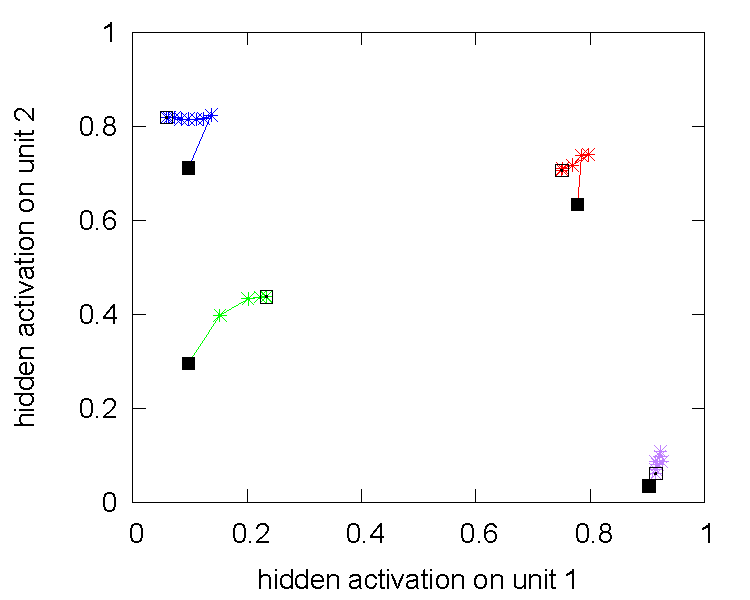
\includegraphics[width=0.45\textwidth]{img/hid-bal-good-init.pdf}  
  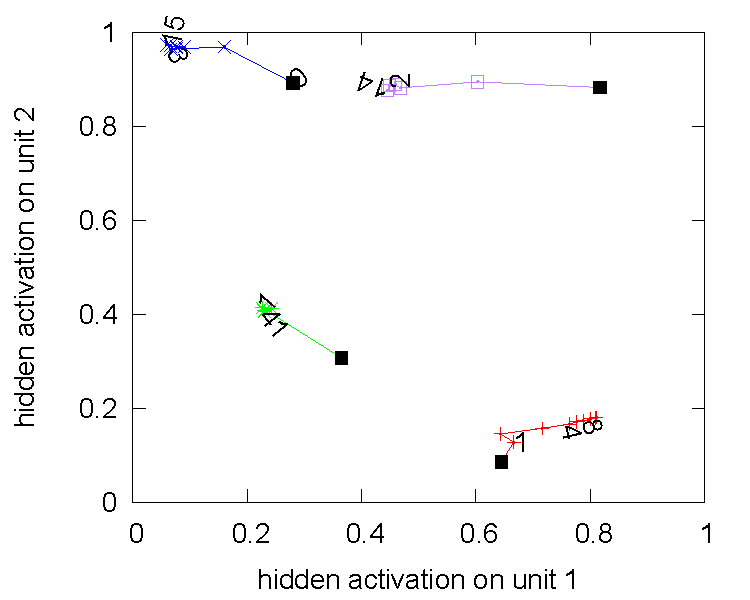
\includegraphics[width=0.45\textwidth]{img/hid-bal-good-convex.pdf}  \\
  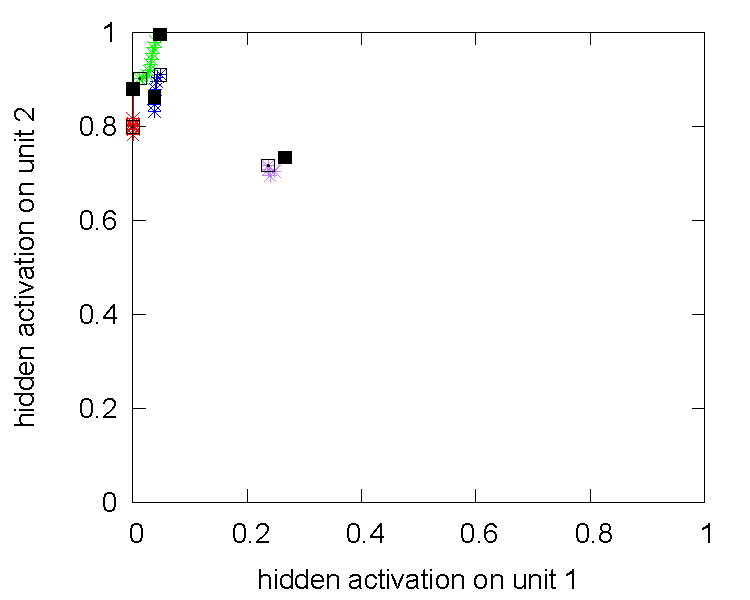
\includegraphics[width=0.45\textwidth]{img/hid-bal-good-step.pdf}  
  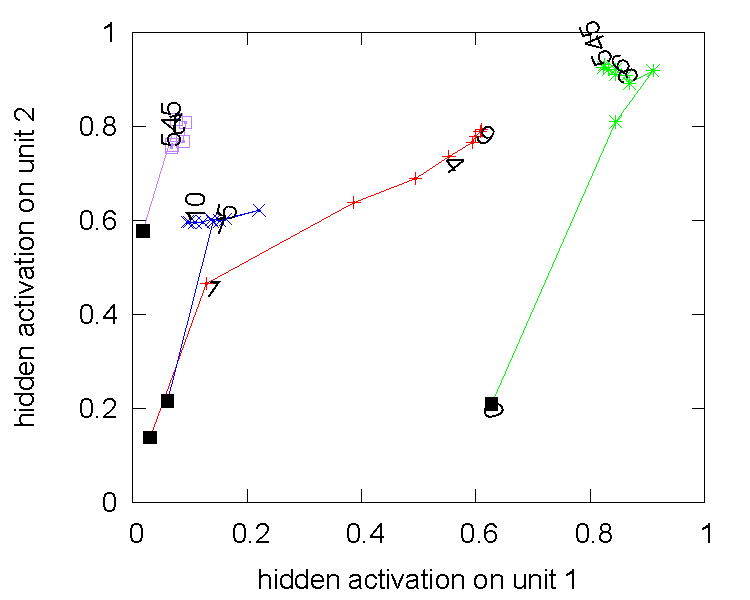
\includegraphics[width=0.45\textwidth]{img/hid-bal-good-stagnation.pdf}  \\ 
  \caption{\emph{BAL} hidden activations on the \emph{4-2-4 encoder} task. The top $2\times2$ are {\bf un}successful networks and the bottom $2\times2$ successful ones. Only the first $\approx 100$ epochs had change in activation.}
  \label{fig:results-hidden-activations-bal}
\end{figure}

\begin{figure}[H]
  \centering
  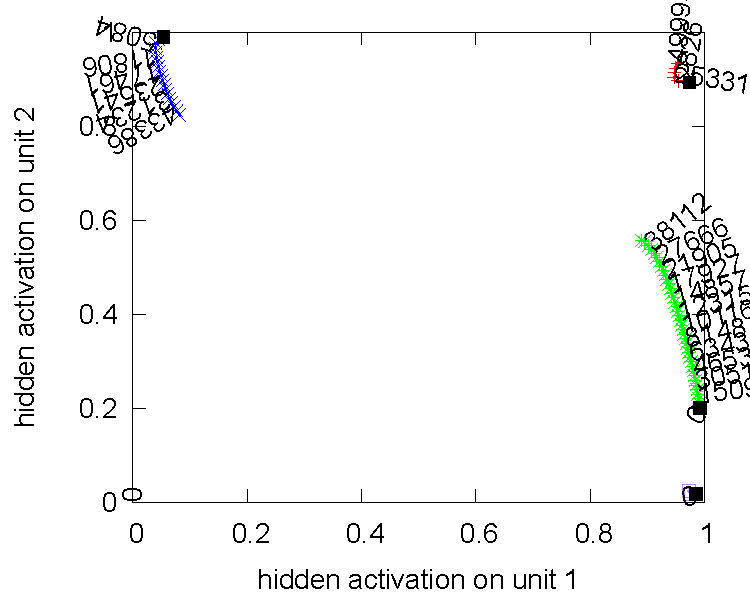
\includegraphics[width=0.45\textwidth]{img/hid-tlr-bad-static.pdf}  
  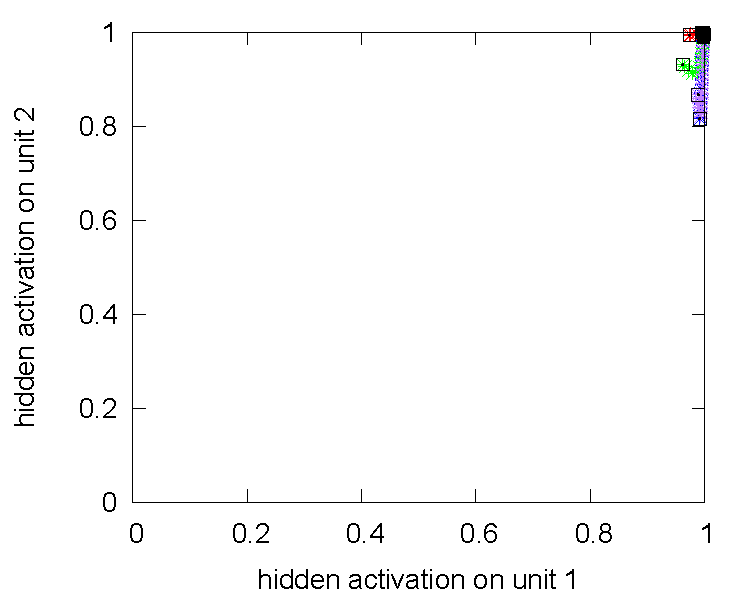
\includegraphics[width=0.45\textwidth]{img/hid-tlr-bad-tiny.pdf}  
  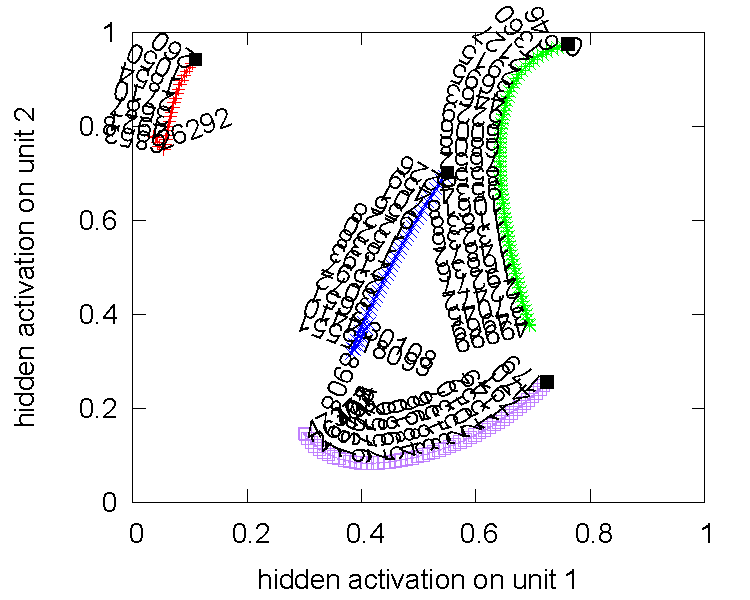
\includegraphics[width=0.45\textwidth]{img/hid-tlr-bad-init.pdf}  
  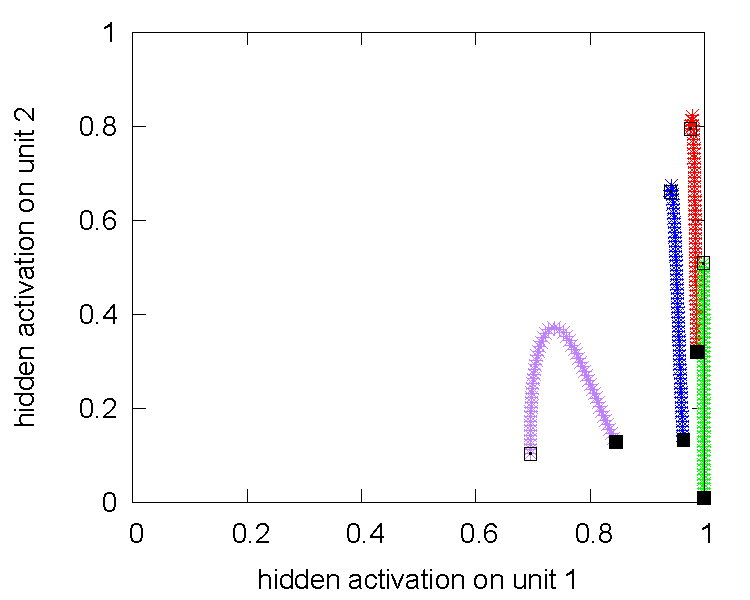
\includegraphics[width=0.45\textwidth]{img/hid-tlr-bad-weird.pdf}  
  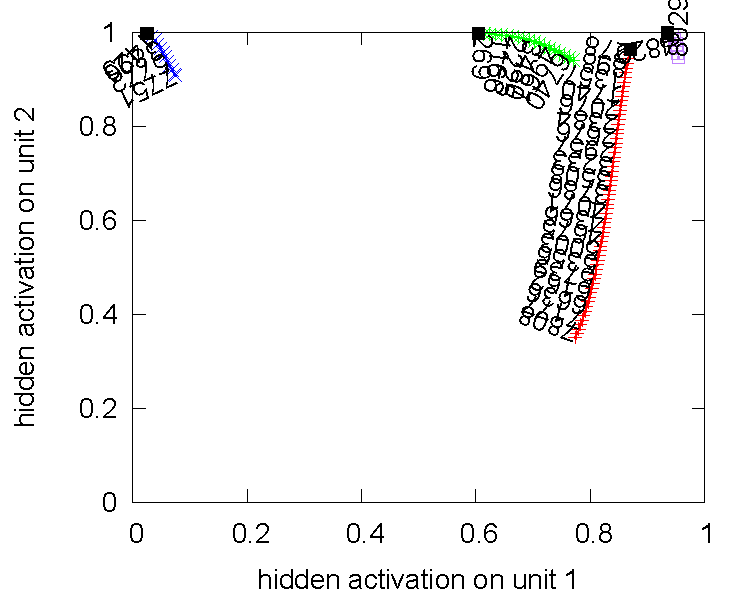
\includegraphics[width=0.45\textwidth]{img/hid-tlr-good-static.pdf}  
  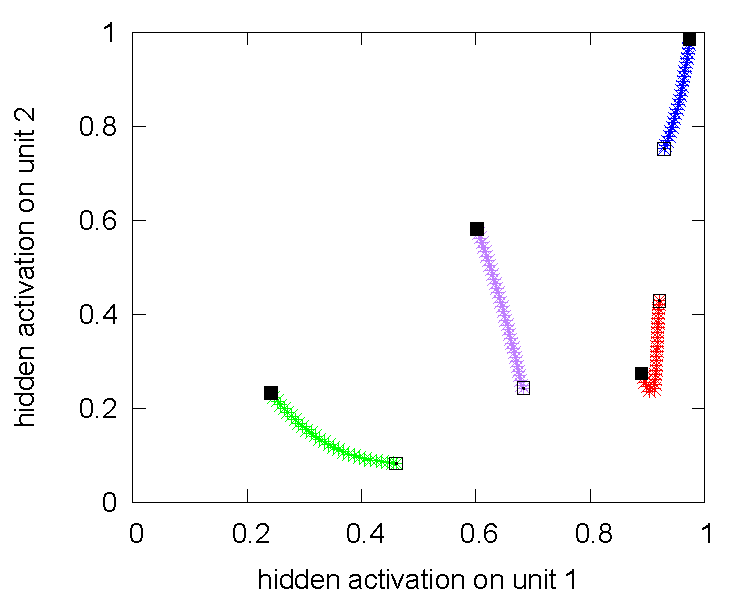
\includegraphics[width=0.45\textwidth]{img/hid-tlr-good-tiny.pdf}  
  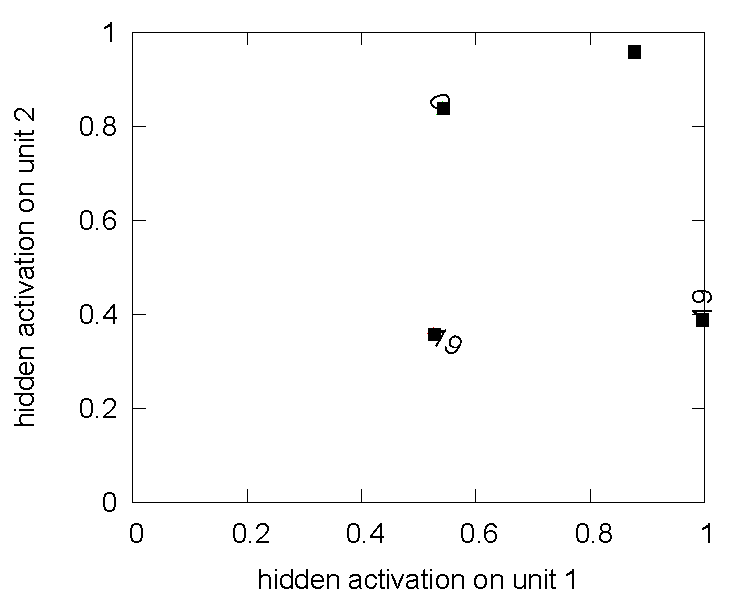
\includegraphics[width=0.45\textwidth]{img/hid-tlr-good-init.pdf}  
  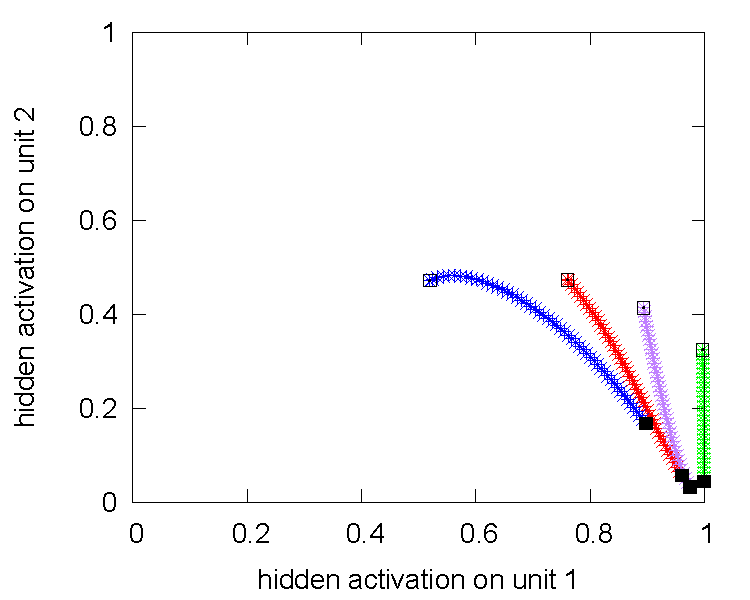
\includegraphics[width=0.45\textwidth]{img/hid-tlr-good-weird.pdf}  
  \caption{\emph{TLR} hidden activations on the \emph{4-2-4 encoder} task. The top $2\times2$ are {\bf un}successful networks and the bottom $2\times2$ successful ones. Only the first $\approx 10000$ epochs had change in activation.}
  \label{fig:results-hidden-activations-tlr}
\end{figure}

%========================================================
\subsubsection{Momentum}
\label{sec:results-momentum} 

Adding momentum~(\ref{sec:our-momentum}) to the basic TLR simulations~(\ref{sec:tlr-auto4}) had no significant effect on network performance as shown in Table~\ref{tab:results-mom-auto4} where for each momentum we take average from all simulations. Only a little improvement in convergence rate was achieved. We ran simulations for range of $\lambda_v$ and $\lambda_h$ values as shown in Figure~\ref{fig:results-tlr-auto4-momentum}. 
\begin{table}[H] 
  \centering
  {\small
    \begin{tabular}{|l|l|}
    \hline
momentum & avg(success) \\
    \hline
0.001  & 0.4419 \\
    \hline
0.003  & 0.4428 \\
    \hline
0.01   & 0.4440 \\
    \hline
0.03   & 0.4464 \\
    \hline
0.1    & 0.4468 \\
    \hline
0.3    & 0.4493 \\
    \hline
    \end{tabular}
  }
  \caption{Comparison of different momentums for TLR on the \emph{4-2-4 encoder} task.} 
  \label{tab:results-mom-auto4}
\end{table}

%======== (3D) L1 x L2 x patSuccF : TLR vs. best momentum =========
%======== (3D) L1 x L2 x epochs : TLR vs. best momentum =========

\begin{figure}[H]
  \centering
  \includegraphics[width=0.49\textwidth]{img/tlr-mom-auto4-success-0-001.pdf}  
  %\includegraphics[width=0.49\textwidth]{img/tlr-mom-auto4-epoch-0-001.pdf}  \\
  \includegraphics[width=0.49\textwidth]{img/tlr-mom-auto4-success-0-3.pdf}  
  %\includegraphics[width=0.49\textwidth]{img/tlr-mom-auto4-epoch-0-3.pdf}  
   \caption{Comparison of momentums $\mu=0.01$ (left) and $\mu=0.3$ (right) for TLR on the \emph{4-2-4 encoder} task.}
  \label{fig:results-tlr-auto4-momentum}
\end{figure}


%============================================================
\subsubsection{Features}
In this section, we analyse the timelines for features $dist_{H}^{FB}$, $dist_{V}^{FB}$, $dist_{H}$ and $matrix\_weight$ introduced in Section~\ref{sec:our-candidates-features}. We compare the values for BAL, TLR and TLR with candidates selection (TLR-can). 

The importance of the distance between forward and hidden activations $dist_{H}^{FB}$ is shown in Figure~\ref{fig:results-candidates-h-fb-d}. We observe that $dist_{H}^{FB}$ settles fast for BAL. This means the network stops learning as the difference $(h^B_j - h^F_j) \approx 0$ renders the weight update in BAL update rule to zero. On the other hand, we see that $dist_{H}^{FB}$ of TLR is not affected in time. This could be contributed to lower magnitude of updates $W^{IH}$ and $W^{OH}$. TLR-can is stationary as it converges in 150 epochs. 

\begin{figure}[H]
  \centering
  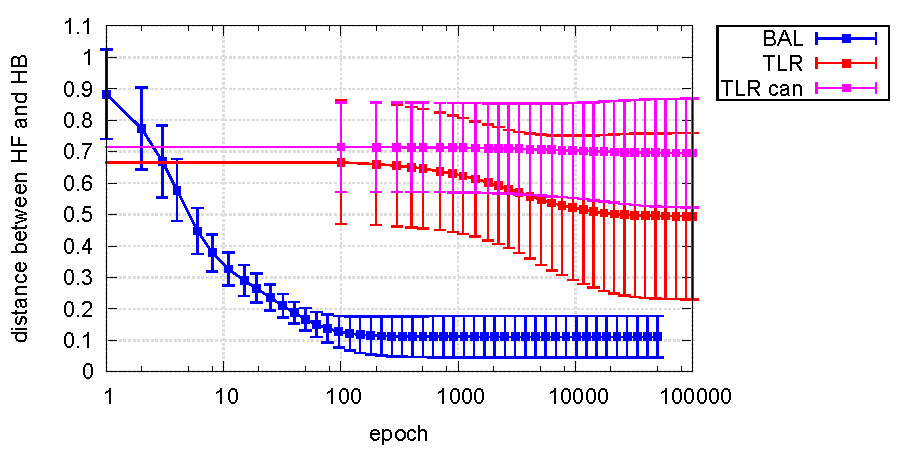
\includegraphics[width=0.6\textwidth]{img/feature-cmp-h-fb-d.pdf}  
   \caption{Comparison of $dist_{H}^{FB}$~(\ref{sec:our-dist-h-fb}) timelines for the {4-2-4 encoder} task.}
  \label{fig:results-candidates-h-fb-d}
\end{figure}

Difference between forward and backward outputs $dist_{V}^{FB}$ is shown in Figure~\ref{fig:results-candidates-o-fb-d}. We see that BAL decreases the difference monotonously and converges to zero. That means the mappings learned by forward and backward weights are same. But, this is not true for TLR. We observe a \emph{rebound} around epoch 4. This could be contributed to $\lambda_h \ll \lambda_v$ as it could greatly increase $|W^{HI}_{ij}|$ and $|W^{HO}_{ij}|$ and therefore activations on output layers change rapidly. After the rebound a convergence phase start which could be explained by settling of $|y^{F} - y^{B}| \approx 0$. This could explain the difference between $y^{F}$ and $x^B$ discussed in Section~\ref{sec:our-o-fb-dist-diff}. 

\begin{figure}[H]
  \centering
  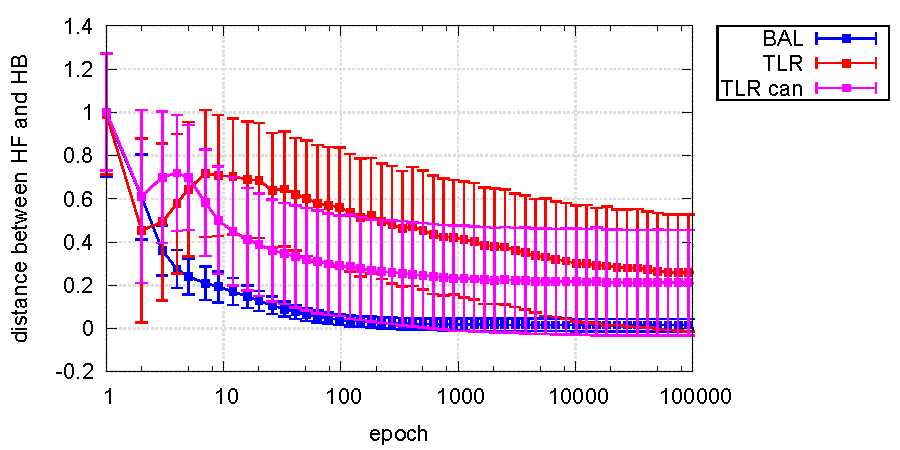
\includegraphics[width=0.6\textwidth]{img/feature-cmp-o-fb-d.pdf}  
   \caption{Comparison of $dist_{V}^{FB}$~(\ref{sec:our-dist-o-fb}) timelines for the {4-2-4 encoder} task.}
  \label{fig:results-candidates-o-fb-d}
\end{figure}

Candidate selection showed that $dist_{H}$ is the primary feature contributing to networks success rate~(\ref{eq:results-candidates-linear-regression}). In Figure~\ref{fig:results-candidates-h-dist} we see that candide selection indeed picks networks with greater $dist_{H}$. We can observe that $dist_{H}$ stagnates through the training phase. This reinforces the importance of proper weight initialization. 

\begin{figure}[H]
  \centering
  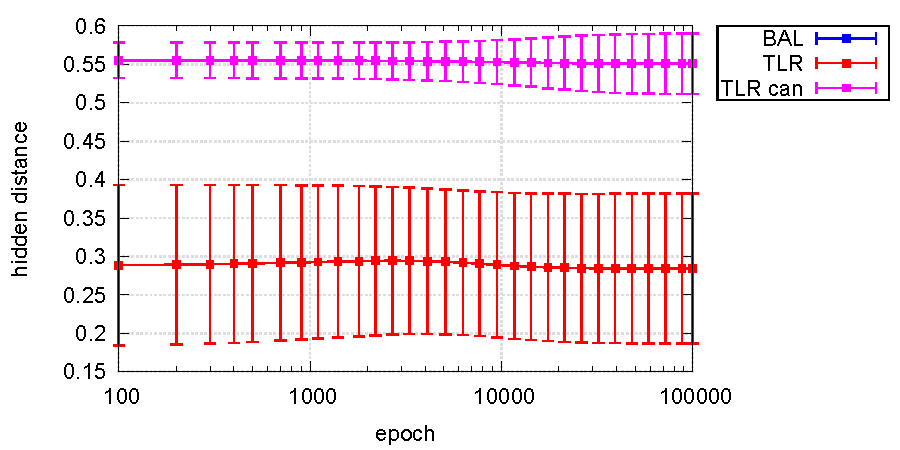
\includegraphics[width=0.6\textwidth]{img/feature-cmp-h-dist.pdf}  
   \caption{Comparison of $dist_{H}$~(\ref{sec:our-h-dist}) timelines for the {4-2-4 encoder} task.}
  \label{fig:results-candidates-h-dist}
\end{figure}

Analysis of the average weight of matrices $matrix\_weight$ in Figure~\ref{fig:results-candidates-m-wei} shows that setting $1 \ll \lambda_v$ leads to greater $matrix\_weight$. We can observe that $matrix\_weight$ is not bounded for TLR and therefore a convenient stopping criteria should be picked. 

\begin{figure}[H]
  \centering
  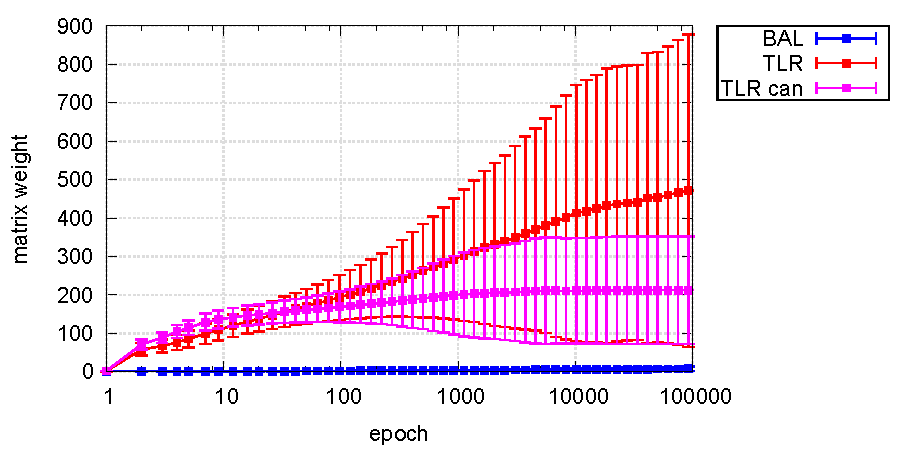
\includegraphics[width=0.6\textwidth]{img/feature-cmp-m-wei.pdf}  
   \caption{Comparison of $matrix\_weight$~(\ref{sec:our-m-wei}) timelines for the {4-2-4 encoder} task.}
  \label{fig:results-candidates-m-wei}
\end{figure}


\subsubsection{Other}

\paragraph{Recirculation BAL.} 
In Figure~\ref{fig:results-bal-recirc-auto4-performance} we see that \emph{BAL-recirc}~(\ref{sec:our-bal-recirc}) achieved lower success rate than BAL on the \emph{4-2-4 encoder} task. In comparison with TLR we see that there is a global maxima at point $\lambda_h = 0.0001$ and $\lambda_v=1.0$. We can therefore conclude that the space of successfull parameters $\lambda_h$ and $\lambda_v$ is bounded. Similar results were achieved for GeneRec as shown in Figure~\ref{fig:results-generec-auto4-performance}.
%======== (3D) L1 x L2 x epochs =========
%======== (3D) L1 x L2 x patSuccF =========
\begin{figure}[H]
  \centering
  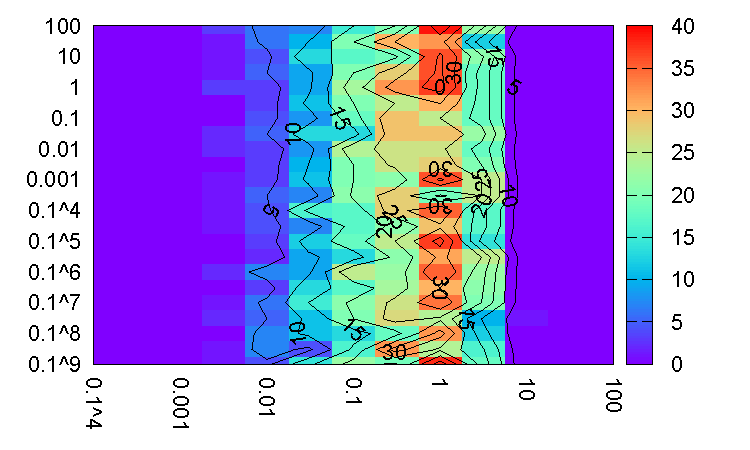
\includegraphics[width=0.49\textwidth]{img/bal-recirc-auto4-success.pdf}   
  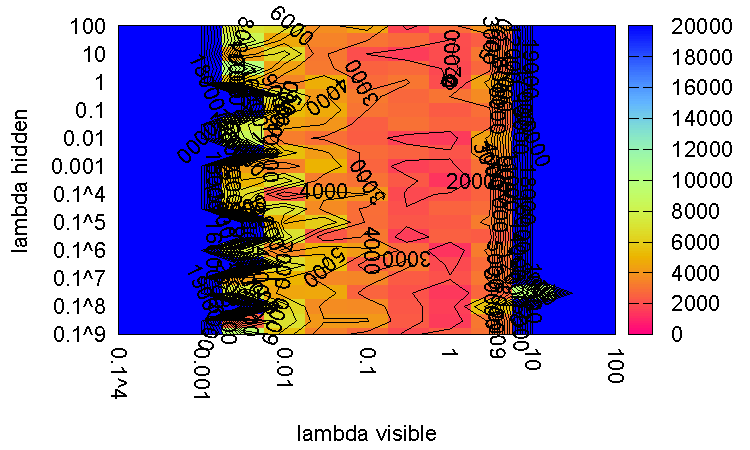
\includegraphics[width=0.49\textwidth]{img/bal-recirc-auto4-epoch.pdf}     
  \caption{BAL-recirc~(\ref{sec:our-bal-recirc}) on the \emph{4-2-4 encoder}. Best success rate  $36\%$ achieved with $\lambda_h = 0.0001$ and $\lambda_v=1.0$.}
  \label{fig:results-bal-recirc-auto4-performance}
\end{figure}
%success lambda_h lambda_v
%33.0 0.0003 1.0
%33.0 0.001 3.0
%34.0 0.01 1.0
%36.0 0.0001 1.0
%36.0 3.0e-05 0.3


\paragraph{GeneRec.} 
As with generalizing of BAL to TLR we tried also generalizing GeneRec using the two learning rates approach. The results in Figure~\ref{fig:results-generec-auto4-performance} show no increase in success rate in comparison with setting $\lambda_v = \lambda_h$, i.e. using the original GeneRec. We can observe that the results are similar with the results of BAL-recirc shown in Figure~\ref{fig:results-bal-recirc-auto4-performance}. Finally, as with BAL-recirc, we can conclude that the success space is bounded.  
%======== (3D) L1 x L2 x epochs =========the
%======== (3D) L1 x L2 x patSuccF =========
\begin{figure}[H]
  \centering
  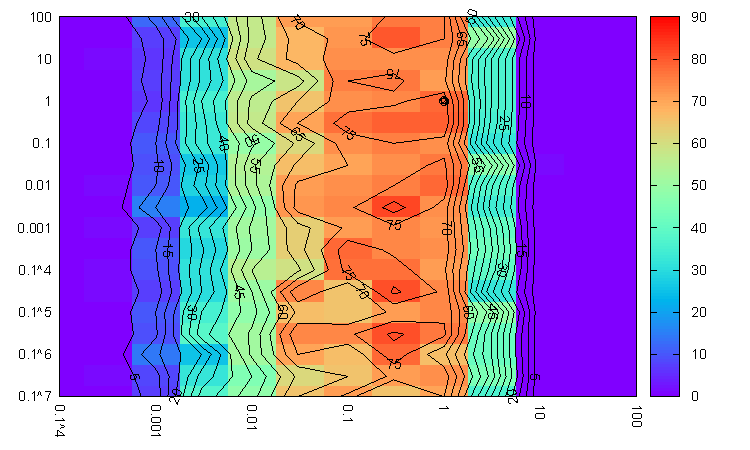
\includegraphics[width=0.49\textwidth]{img/generec-auto4-success.pdf}   
  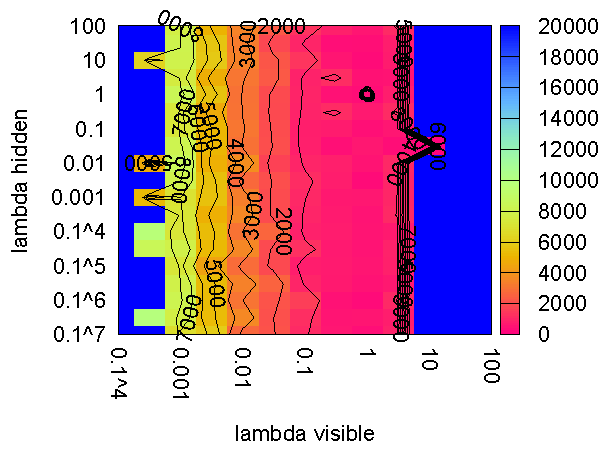
\includegraphics[width=0.49\textwidth]{img/generec-auto4-epoch.pdf}     
  \caption{GeneRec~(\ref{sec:models-generec}) success rate and convergence time on the \emph{4-2-4 encoder} task with $\sigma = 2.3$ and $\mu = 0.0$. Best result $83\%$ achieved with $\lambda_h = 0.3$ and $\lambda_v=1.0$.}
  \label{fig:results-generec-auto4-performance}
\end{figure}

%77.0 1.0 0.1
%78.0 1.0 0.3
%81.0 0.3 0.3
%83.0 0.3 1.0


\subsubsection{Conclusion} 
\label{sec:tlr-auto4-conclusion} 

\label{sec:tlr-auto4-hypothesis} 
The results in this chapter suggest a hypothesis why TLR outperforms BAL on the \emph{4-2-4 encoder task}. The reason is that the hidden activations settle before $W^{HO}$ and $W^{HI}$ adapt to them. This is explained by the fact that forward and backward hidden activations become same to fast~(\ref{sec:tlr-auto4-hidden},~\ref{sec:our-hidden-activation}) and moreover, weight initialization could help this~(\ref{fig:results-tlr-auto4-epoch}). The first issue is solved by setting $\lambda_h \ll \lambda_h$ what adds epochs to the training phase. The second issue is solved by candidate selection which prevents initializing hidden activations close to each other. 

